%%
%% This is file `sample-manuscript.tex',
%% generated with the docstrip utility.
%%
%% The original source files were:
%%
%% samples.dtx  (with options: `manuscript')
%% 
%% IMPORTANT NOTICE:
%% 
%% For the copyright see the source file.
%% 
%% Any modified versions of this file must be renamed
%% with new filenames distinct from sample-manuscript.tex.
%% 
%% For distribution of the original source see the terms
%% for copying and modification in the file samples.dtx.
%% 
%% This generated file may be distributed as long as the
%% original source files, as listed above, are part of the
%% same distribution. (The sources need not necessarily be
%% in the same archive or directory.)
%%
%% Commands for TeXCount
%TC:macro \cite [option:text,text]
%TC:macro \citep [option:text,text]
%TC:macro \citet [option:text,text]
%TC:envir table 0 1
%TC:envir table* 0 1
%TC:envir tabular [ignore] word
%TC:envir displaymath 0 word
%TC:envir math 0 word
%TC:envir comment 0 0
%%
%%
%% The first command in your LaTeX source must be the \documentclass command.
\documentclass[manuscript,screen,review]{acmart}

%%
%% \BibTeX command to typeset BibTeX logo in the docs
\AtBeginDocument{%
  \providecommand\BibTeX{{%
    \normalfont B\kern-0.5em{\scshape i\kern-0.25em b}\kern-0.8em\TeX}}}

%% Rights management information.  This information is sent to you
%% when you complete the rights form.  These commands have SAMPLE
%% values in them; it is your responsibility as an author to replace
%% the commands and values with those provided to you when you
%% complete the rights form.
\setcopyright{acmcopyright}
\copyrightyear{2018}
\acmYear{2018}
\acmDOI{XXXXXXX.XXXXXXX}

%% These commands are for a PROCEEDINGS abstract or paper.
\acmConference[Conference acronym 'XX]{Make sure to enter the correct
  conference title from your rights confirmation emai}{June 03--05,
  2018}{Woodstock, NY}
\acmPrice{15.00}
\acmISBN{978-1-4503-XXXX-X/18/06}


%%
%% Submission ID.
%% Use this when submitting an article to a sponsored event. You'll
%% receive a unique submission ID from the organizers
%% of the event, and this ID should be used as the parameter to this command.
%%\acmSubmissionID{123-A56-BU3}

%%
%% For managing citations, it is recommended to use bibliography
%% files in BibTeX format.
%%
%% You can then either use BibTeX with the ACM-Reference-Format style,
%% or BibLaTeX with the acmnumeric or acmauthoryear sytles, that include
%% support for advanced citation of software artefact from the
%% biblatex-software package, also separately available on CTAN.
%%
%% Look at the sample-*-biblatex.tex files for templates showcasing
%% the biblatex styles.
%%

%%
%% The majority of ACM publications use numbered citations and
%% references.  The command \citestyle{authoryear} switches to the
%% "author year" style.
%%
%% If you are preparing content for an event
%% sponsored by ACM SIGGRAPH, you must use the "author year" style of
%% citations and references.
%% Uncommenting
%% the next command will enable that style.
%%\citestyle{acmauthoryear}

%%
%% end of the preamble, start of the body of the document source.
\begin{document}

%%
%% The "title" command has an optional parameter,
%% allowing the author to define a "short title" to be used in page headers.
\title{Journal \#3}

%%
%% The "author" command and its associated commands are used to define
%% the authors and their affiliations.
%% Of note is the shared affiliation of the first two authors, and the
%% "authornote" and "authornotemark" commands
%% used to denote shared contribution to the research.
\author{SangHyun Byun}
%%\authornote{Both authors contributed equally to this research.}
\email{sbyun@uccs.edu}
\orcid{1234-5678-9012}
\affiliation{%
  \institution{University of Colorado Colorado Springs}
  \city{Colorado Springs}
  \state{Colorado}
  \country{USA}
  \postcode{80918}
}


%%
%% By default, the full list of authors will be used in the page
%% headers. Often, this list is too long, and will overlap
%% other information printed in the page headers. This command allows
%% the author to define a more concise list
%% of authors' names for this purpose.
\renewcommand{\shortauthors}{SangHyun, et al.}

%%
%% The abstract is a short summary of the work to be presented in the
%% article.
\begin{abstract}
  
\end{abstract}

%%
%% The code below is generated by the tool at http://dl.acm.org/ccs.cfm.
%% Please copy and paste the code instead of the example below.
%%

%%
%% This command processes the author and affiliation and title
%% information and builds the first part of the formatted document.
\maketitle

\section{survey paper}
In this section, I show the list of survey papers related to federated learning and provide critically and creatively read.

\begin{figure*}[t]
\centering
{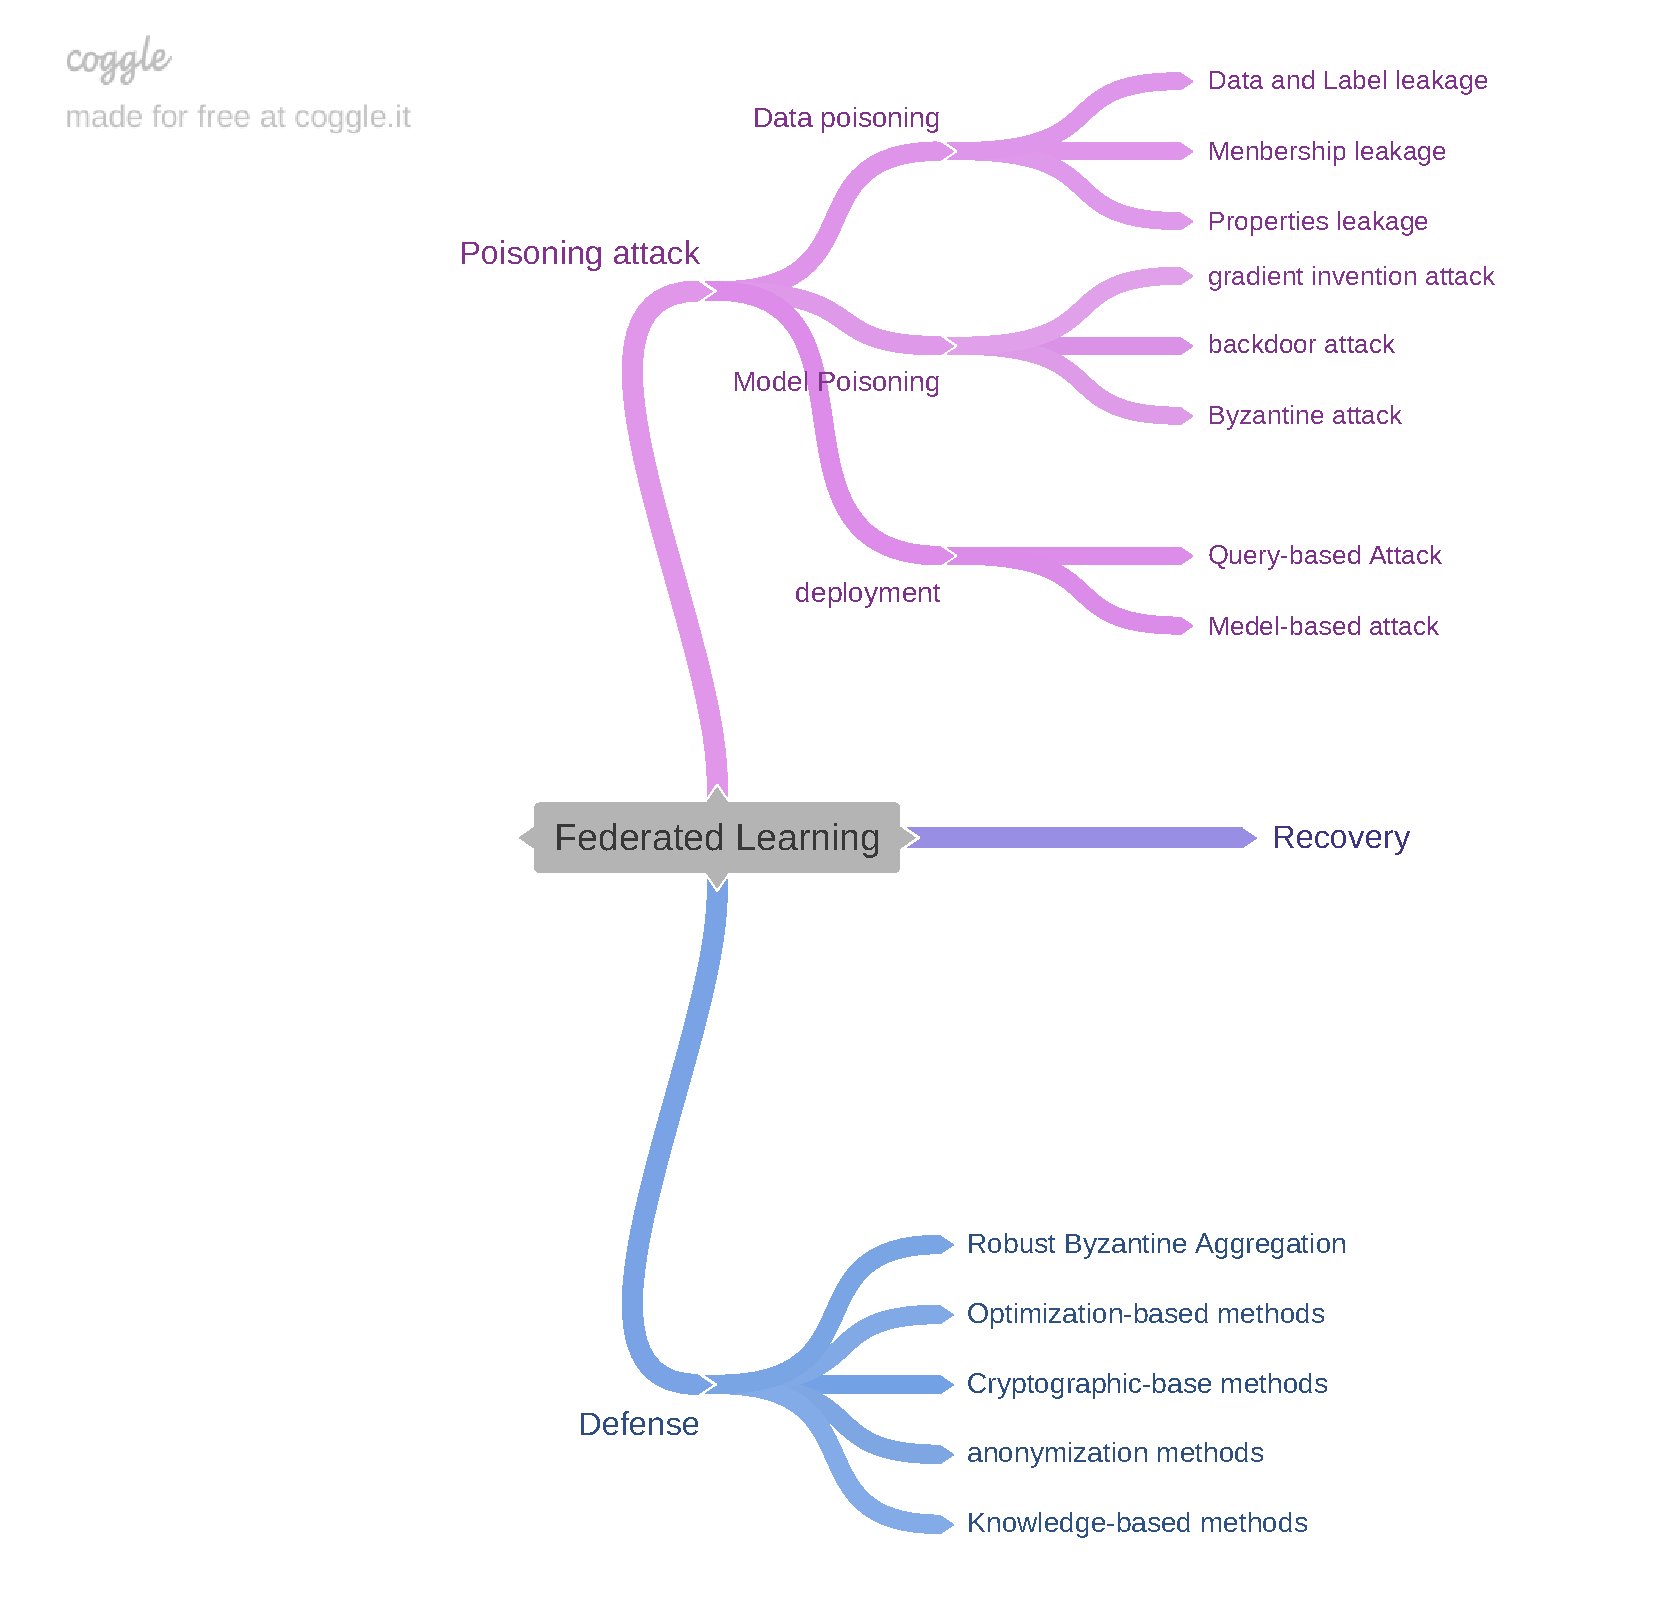
\includegraphics [width=1\textwidth]{graphics/maps}}
\caption{Maping of federated learning security and privacy
}
\label{fig:SPSC}
\end{figure*}



1. survey~\cite{mothukuri2021survey}*
This survey paper aims at the security and privacy of federated learning. Federated learning addresses solutions for traditional machine learning methods with data privacy and security. It highlights the shift from a centralized machine learning concept to a decentralized machine learning concept (federated learning), in which clients' devices are only allowed to access raw data and then trained it through global model. Most challenges in cloud-based traditional machine learning rely on a centralized system to collect data and train, which means that poses challenges in data privacy, security, and efficiency. Federated learning provides solutions to these challenges. It decentralizes the learning process through clients' devices. Only the server gains the outcomes of training data and aggregates the outcomes of training data from each device. Federated learning addresses fundamental problems related to data privacy, ownership, and data locality. Even though each devices only access the raw data and trained in devices, server does not know raw data and training process, which means that enhances privacy and security, aligning with merging data protection laws. However, it has new security and privacy challenges to share model parameters and to conduct numerous training iterations and potential security breaches and vulnerabilities in communication issues.       

This survey paper is a good paper for me to understand the concern of federated learning and research objectives of federated learning. the goal is to promote security-related research and advance federated learning. Reference papers is 252, which is many paper and the number of citations is 632.

2. survey~\cite{li2021survey}*
This survey paper shows a critical concern about machine learning and solutions to those concerns. The limitation of the traditional machine learning concept relies on centralized systems for the computational learning process without privacy and security. Federated learning provides the decentralized machine learning concept that each client tries to train the global model from raw data that the client only accesses. Global model updates that does not include personal information should deliver to a central server. It can aggregate the global model updates. It is beneficial for machine learning to preserve the privacy of data. Nowadays, many countries have enhanced data protection laws or regulations, which means that it is important to provide data privacy and user privacy. machine learning requires a mass dataset including sensitive data. It shows that new security and privacy challenges particularly sharing the model parameters and global models among clients. 

This paper was a good survey paper 2 years ago. This paper provides good reference paper numbers is 
 569. It was published in IEEE Transactions on Knowledge and Data Engineering.     

3. survey~\cite{yin2021comprehensive}

4. survey~\cite{zhang2021survey}

5. survey~\cite{lyu2020threats}

6. survey~\cite{truong2021privacy}

7. survey~\cite{blanco2021achieving}

8. survey~\cite{liu2022privacy}

9. survey~\cite{rasha2023federated}

10. survey~\cite{zhang2023survey}*
This survey paper explains the emergence of trustworthy federated learning with the privacy concerns and security issues in machine learning. The key points of this survey paper are divided into several points such as trustworthy AI, trustworthy federated learning, vulnerabilities in federated learning, core aspects of federated learning trustworthiness, the framework of trustworthy federated learning, and threats and defense methods in recent years. First, trustworthy AI and federated learning have adversarial attacks to affect learning outcomes. Specifically, AI has concerns about the potential privacy and security issue and then Federated learning provides more privacy and security for machine learning in distributed environments. However, while federated learning is a valuable approach, it is vulnerable to adversarial attacks, which can compromise model integrity and data. The federated learning process will be addressed to ensure trustworthiness for federated learning against data processing, model training, and deployment during the federated learning process. This paper shows three core federated learning trustworthiness including Privacy to protect personal information, Robustness to ensure stability and reliability, and Security to protect against unauthorized access. Finally, it discusses threats and defense methods related to federated learning such as data and label leakage, gradient attacks, model poisoning, and Byzantine attacks and inference attacks.

This paper is a good survey paper for me to categorize well and to organize many contents of federated learning. However, it includes a lot of content, which means that it is complicated to understand the contribution of the survey. The reference papers are 262. It will be increasing the citation number.    


11. survey~\cite{xia2023poisoning}*
This survey paper shows security and privacy issues in federated learning. These attacks can severely poison global models and enable malicious activities to have negative effects on model convergence or manipulate prediction outcomes. Defending poisoning attacks is an urgent and challenging task. However, it is difficult to review the poisoning attacks and privacy-preserving defense strategies. This survey paper offers an extensive and current exploration of poisoning attacks and the corresponding defense methods with federated learning. This paper should categorize the poisoning attacks based on current existing methods and different poisoning targets, but the poisoning result is a poisoning global model. Subsequently, this paper provides the distinctions and connections among various attack categories. Additionally, it classifies defense strategies against poisoning attacks. Finally, the issue of privacy-preserving to protect the original data from poisoning attacks such as byzantine robust aggregation algorithm, model analysis, and verification. Each method has its strengths and weaknesses depending on the poisoning attack.      

This paper is a recent survey paper and the citation number is 3. I think it is important which Journal survey paper is published. The most important thing is the survey direction and how many reference papers the survey paper includes. the reference papers in this paper are 65. The topic is specific, which means that it is difficult to find new attacks and new defense papers.   



12. survey~\cite{gosselin2022privacy}*
This survey paper described privacy and security concerns of federated learning in recent years. This paper discusses that it is important for machine learning approaches to protect in addressing complex problems with several poisoning attacks, such as data poisoning, model poisoning, and outcome poisoning. The paper highlights why change from centralized machine learning to decentralized machine learning defined as federated learning to provide privacy concerns, legal constraints, and increase the data volume. Federated learning allows to aggregation of the training model from each client without sharing raw data, preserving privacy and communication cast. However, It presents challenges, such as maintaining performance with non-identically and independently distributed (non-IID) local raw data. 
Federated Learning addresses the challenges to collaborate machine learning model. Federated Learning provides privacy advantages for data and users. However, FL remains susceptible to attacks that is able to effect model integrity and data security. This paper mentions that it categorized existing research through various aspects of FL with a limited focus on federated learning security and privacy. This paper aims to conduct a comprehensive study on security and privacy risk in federated learning and provides formal definitions, attacks, defense and future challenges. 

This paper is a recent survey paper and the citation number is 17. It is similar than that paper~\cite{xia2023poisoning} because of citation number and reference papers. reference papers are 67. 




%%
%% The acknowledgments section is defined using the "acks" environment
%% (and NOT an unnumbered section). This ensures the proper
%% identification of the section in the article metadata, and the
%% consistent spelling of the heading.


%%
%% The next two lines define the bibliography style to be used, and
%% the bibliography file.
\bibliographystyle{ACM-Reference-Format}
\bibliography{bibliography}

%%
%% If your work has an appendix, this is the place to put it.
\appendix



\end{document}
\endinput
%%
%% End of file `sample-manuscript.tex'.
